\documentclass{article}
\usepackage[utf8]{inputenc}
\usepackage[spanish]{babel}
\usepackage{ifpdf}
\usepackage{hyperref}
\usepackage{subcaption}
\usepackage{graphicx}
\usepackage{caption}
\usepackage{mathtools}
\title{Equipos e Instalaciones Eléctricas Aeronáuticas}
\author{Leandro Marsó}
\date{2015}
\ifpdf
\hypersetup{
    pdfauthor={Leandro Marsó},
    pdftitle={Equipos e Instalaciones Eléctricas Aeronáuticas},
}
\fi

% Para cambiar los nombres por defecto:
% Babel traducía table como cuadro. Yo lo cambio para tabla:
\addto\indexspanish{%
  \renewcommand{\indexname}%
    {Programa de la materia}%
}

\begin{document}
\maketitle
\pagebreak
\tableofcontents
\pagebreak
	\section{Electrostática}
La electrostática es el análisis de fenómenos en que las partículas con carga eléctrica se encuentran en reposo. O por decirlo de otra forma, con fuentes y campos eléctricos que no varían su valor según pasa el tiempo.

	\subsection{Carga eléctrica}
A partir de una serie de experimentos sencillos, Benjamín Franklin (1706-1790) determinó que existen dos tipos de cargas eléctricas, a las que dio el nombre de positiva y negativa. Los electrones tienen carga negativa y los protones positiva. Para comprobar la
existencia de ambos tipos de carga, realizamos el experimento Nº 1.

La unidad de carga más pequeña e conocida en la naturaleza, es la carga de un electrón (-e) o de un protón (+e), con una magnitud de
$$ e = 1,602 18 \times 10^{19} C$$

\subsubsection*{Experimento Nº 1}
Tomamos una cinta de teflón de aproximadamente 40cm y la sostenemos por la mitad. Notamos que la cinta cae libremente, con sus dos extremos muy cerca el uno del otro. Luego frótela varias veces con un material de lana, hasta ver que ambos extremos ya no se tocan mas al colgar, e incluso se separan formando una \textbf{v} invertida. Si luego acercamos a la cinta de teflón el mismo material de lana que utilizamos para frotar, observaremos que la cinta se eleva atraída por la lana. Esta observación demuestra que la cinta de teflón y la lana tienen dos tipos diferentes de carga. Con base en estas observaciones, se puede concluir que \textbf{cargas de un mismo signo se repelen y cargas de signos opuestos se atraen}.

	\subsection{Leyes y reglas de la electrostática}
	\subsubsection*{Ley de Coulomb}
En el siglo XVIII, el físico e ingeniero Charles Coulomb propuso un experimento que le permitió precisar las siguientes cuatro observaciones:

\begin{itemize}
\item Los cuerpos cargados sufren una fuerza de atracción o repulsión al aproximarse.
\item El valor de dicha fuerza es proporcional al producto del valor de sus cargas.
\item La fuerza es de atracción si las cargas son de signo opuesto y de repulsión si son del mismo signo.
\item La fuerza es inversamente proporcional al cuadrado de la distancia que los separa.
\end{itemize}

Coulomb determinó el valor de la fuerza que existe entre dos partículas cargadas como se muestra en la figura \ref{fig:cargasneg}:

\begin{center}
	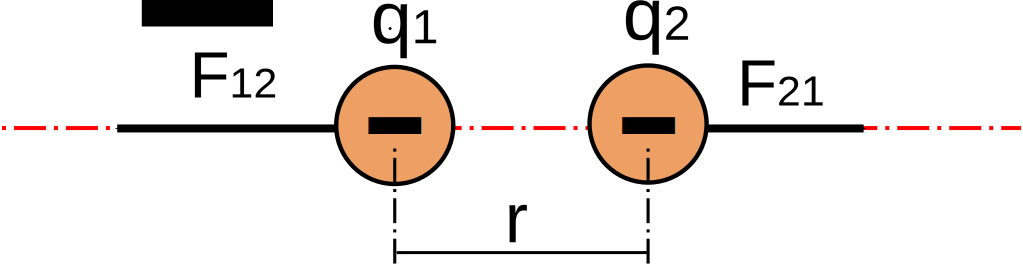
\includegraphics[scale=0.25]{figuras/cargasneg.pdf}
	\captionof{figure}{\emph{Dos partículas con carga eléctrica experimentan una fuerza debido a la existencia de la otra. Coulomb con su experimento, determinó las magnitudes de estas fuerzas}.}
\label{fig:cargasneg}
\end{center}

Coulomb sintetizó los resultados de su experimento con la siguiente ecuación:

\begin{equation}
|\vec{F}_{12}| = |\vec{F}_{21}| = \frac{q_1q_2}{r^2}k
\label{eq:CoulombForce}
\end{equation}

Utilizando la ecuación \ref{eq:CoulombForce}, podemos decir que: 

\begin{itemize}
\item $q_1$ y $q_2$ son los valores de dos cargas puntuales, en el S.I. se mide en Coulomb
\item $r$ es la separación entre las cargas, en metros para el S.I.
\item $\vec{F}_{12}$ es la fuerza sobre la carga $q_1$ debido a la existencia de la carga $q_2$, y $\vec{F}_{21}$ es la fuerza sobre la carga $q_2$ debido a la existencia de $q_1$. Esta fuerza se mide en Newtons en el S.I.. Con $|\vec{F}_{12}|$ queremos decir que esta fórmula nos dá el valor de la fuerza, pero nada dice de la \textbf{dirección y sentido} de la fuerza, la cual se puede determinar por el signo de las cargas (se repelen o se atraen, es decir \textbf{el sentido}) y por la línea imaginaria que une a las cargas y de longitud $r$, que nos da \textbf{la dirección}.
\item $k$ es una constante conocida como \textbf{constante de Coulomb}. 
\end{itemize}

%	\subsection{Fenómenos electrostáticos}

\subsubsection*{Apéndice}
El valor de la constante de Coulomb depende del medio en que se encuentren las partículas (vacío, aire, agua, etc) y de la elección de las unidades. La unidad de carga del Sistema Internacional (SI) es el \textbf{coulomb} (C). La constante de Coulomb para el vacío (la nombramos como $k_e$) en unidades del SI tiene el valor
$$k_e = 8,9876 \times 10^9 N \cdot m^2/C^2$$

Además, esta constante se expresa como

$$k_e = \frac{1}{4\pi\epsilon_0} $$ 

donde $\epsilon_0$ (letra griega minúscula epsilon) es el valor de la permitividad del vacío y su valor es $8,85418 \times 10^{-12}$ Faradios/metro (F/m).

Generalizando, decimos que $\epsilon = \epsilon_0\epsilon_r$, y $\epsilon_r$ es la permitividad dialéctrica relativa del medio en que se encuentren. Por ejemplo el $\epsilon_r$ del vacío es $1$, el de la mica es de $5,4$ y el del papel aprimadamente $50$. 


	\subsection{Campo eléctrico}
El concepto de campo lo desarrolló Michael Faraday (1791-1867) en relación con las fuerzas eléctricas. Faraday planteó que existe un campo eléctrico en la región del espacio que rodea a un objeto con carga: la carga fuente. Cuando otro objeto con carga —la carga de prueba— entra en este campo eléctrico, una fuerza eléctrica actúa sobre él. 

Para ejemplificar, observe la figura \ref{fig:campo}, que muestra una pequeña carga de prueba positiva $q_i$ colocada cerca de un segundo objeto con una carga positiva $Q$ mucho mayor. El campo eléctrico provocado por la carga fuente en la carga de prueba es la fuerza eléctrica que actúa sobre la carga de prueba, dividida por el valor $q_i$:
$$
\vec{E}\equiv \frac{\vec{F}_e}{q_i}
$$

\begin{center}
	\includegraphics[scale=0.50]{figuras/campo-1.png}
	\captionof{figure}{\emph{Una pequeña carga de prueba positiva $q_i$ colocada en el punto P cerca de un objeto con una carga positiva $Q$ mucho mayor experimenta un campo eléctrico E en el punto P establecido por la carga fuente $Q$.}}
\label{fig:campo}
\end{center}

El vector $\vec{E}$ en unidades S.I. es: newtons por coulomb (N/C). Observe que $\vec{E}$ es el campo producido por una carga o distribución de carga separada de la carga de prueba; no es el campo producido por la propia carga de prueba, además observe que la existencia de un campo eléctrico es una propiedad de su fuente; la presencia de una carga de prueba no es necesaria para que el campo exista. La carga de prueba sirve como detector del campo eléctrico. La dirección de $\vec{E}$, como se muestra en la figura \ref{fig:campo}, es la dirección de la fuerza que experimenta una carga de prueba positiva cuando es colocada en el campo; \textbf{existe un campo eléctrico en un punto si una carga de prueba en dicho punto experimenta una fuerza eléctrica}.


%Antes de Faraday la idea de las líneas de fuerza se había tratado como un artificio matemático. Estas líneas de fuerza ya se habían definido de la siguiente forma: supongamos que hay una fuerza entre dos tipos de partículas, por ejemplo, eléctricas. Sabemos que si son de cargas iguales se repelen, mientras que si sus cargas son opuestas se atraen. Consideremos una partícula eléctrica positiva (Figura 8(a)), que llamaremos 1. Tomemos ahora otra partícula, la 2, también positiva, pero de carga mucho menor que la 1. A esta partícula 2 la llamaremos de prueba, pues con ella veremos qué pasa en el espacio alrededor de la partícula 1. La fuerza entre ellas se muestra en la figura. Ahora dejemos que la partícula de prueba se mueva un poco. Debido a que es repelida por la 1 se alejará y llegará a una nueva posición que se muestra en la figura 8(b). Si se vuelve a dejar que la partícula de prueba se mueva un poco llegará a otra posición, y así sucesivamente. La trayectoria que sigue la partícula de prueba al moverse en la forma descrita es una línea de fuerza. Nos damos cuenta de que la fuerza que experimenta la partícula de prueba es siempre tangente a la línea de fuerza. Ahora podemos repetir la experiencia colocando la partícula de prueba en otro lugar y así formar la línea de fuerza correspondiente. De esta manera podemos llenar todo el espacio que rodea a la partícula 1 de líneas de fuerza, y nos percatamos de que todas ellas salen de la partícula 1. http://bibliotecadigital.ilce.edu.mx/sites/ciencia/volumen3/ciencia3/112/htm/sec_8.htm

\pagebreak


%	\subsection{Inducción y líneas de fuerza}
%	\subsection{Trabajo y energía eléctrica}
\subsection{Potencial eléctrico}
\subsubsection{Diferencia de potencial y potencial eléctrico en campos eléctricos uniformes}

Cuando se coloca una carga de prueba $q_i$ en un campo eléctrico \textbf{E} producido por alguna una distribución uniforme de carga fuente, la fuerza eléctrica que actúa sobre ella es $q_iE$. La fuerza $q_iE$ es conservativa, ya que la fuerza entre cargas descrita por la ley de Coulomb es conservativa. Cuando se traslada la carga de prueba por algún agente externo en el campo, el trabajo consumido por el campo en la carga es igual al trabajo invertido por el agente externo que origina el desplazamiento, pero con signo negativo. Esto es semejante a lo que se presenta cuando se levanta un objeto con masa en un campo gravitacional: el trabajo invertido por el agente externo es igual pero de signo opuesto a el trabajo consumido por la fuerza gravitacional.

\begin{center}
	\includegraphics[scale=0.25]{figuras/distribucion-uniforme.pdf}
	\captionof{figure}{\emph{Distribución uniforme de cargas crean un campo eléctrico uniforme}.}
\label{fig:cargasneg}
\end{center}

Si por ejemplo,  hasta un lugar cercano del origen del campo, la energía potencial de esta carga de prueba en este campo es $U$.

Para un desplazamiento de distancia $d$ de una carga puntual $q_i$ inmersa en un campo eléctrico uniforme, el trabajo realizado por un campo eléctrico sobre la misma es $Fd = q_i\vec{E}d$. Conforme el campo consume esta cantidad de trabajo, la energía potencial del 
sistema carga-campo cambia en una cantidad $ \Delta U = -q_i \vec{E}d$.

Para un desplazamiento de $d$ de la carga desde un punto \textbf{A} al punto \textbf{B} el cambio en energía potencial del sistema es:
$$ \Delta U = -q_i (E_B - E_A)d$$

	\subsection{Diferencia de potencial}
Si dividimos el cambio de energía potencial, por la carga de prueba obtenemos lo que se conoce como \textbf{diferencia de potencial} entre el punto A y B, debido al campo eléctrico. La ecuación entonces es:

$$ \Delta V = \frac{\Delta U}{q_i} = -(E_B - E_A)d $$ 

\subsection{Capacitores}
Los capacitores son uno de los tres elementos simples de circuitos que se interconectan mediante alambres para formar un circuito eléctrico. Los circuitos eléctricos son la base de la gran mayoría de los dispositivos que se utilizan el día de hoy. 
Los capacitores, dispositivos que almacenan carga eléctrica.


Los capacitores se usan de manera regular en diversidad de circuitos eléctricos. Por ejemplo, se usan para sintonizar la frecuencia de los receptores de radio, en filtros de fuentes de energía eléctrica, y para eliminar las chispas en los sistemas de magnetos  para el encendido de los motores alternativos de aviación.

\subsubsection*{Definición de la capacitancia}

Considere dos conductores como se observa en la figura \ref{fig:capa12}. Esta combinación de dos conductores se conoce como capacitor. Los conductores son las placas. Si los conductores llevan carga de igual magnitud y signo opuesto existe una diferencia de potencial $\Delta V$ entre ellos.


\begin{center}
	\includegraphics[scale=0.25]{figuras/capacitor12v}
	\captionof{figure}{\emph{Capacitor de placas paralas conectado a una batería de 12V}.}
\label{fig:capa12}
\end{center}

¿Qué determina cuánta carga existe en las placas de un capacitor para cierto voltaje? Los experimentos han demostrado que la cantidad de carga $Q$ en un capacitor es linealmente proporcional a la diferencia de potencial entre los conductores; es decir $Q \propto \Delta V$

La constante de proporcionalidad depende de la forma y separación de los conductores. Esta relación se escribe como $Q = C \Delta V$ si define la capacitancia de la siguiente manera:

La \textbf{capacitancia} C de un capacitor se define como la relación de la magnitud de
la carga en cualquiera de los conductores a la magnitud de la diferencia de potencial
entre dichos conductores:
$$C \equiv \frac{Q}{\Delta V}$$


La unidade del SI para capacitancia es el \textbf{Farad} (F), y se define como $$1~\textrm{F} = 1~ \textrm{C}/\textrm{V}$$



\pagebreak
\section{Corriente Eléctrica}
\subsubsection{Naturaleza de la corriente eléctrica}
Consideremos un cuerpo A cargado negativamente debido a un exceso de electrones y un cuerpo B en estado neutro (figura \ref{fig:corriente}).

Unamos estos dos cuerpos por un hilo conductor. Los electrones en exceso en A atraviesan el hilo conductor hacia el cuerpo B hasta que los dos cuerpos equilibran sus cargas. Este flujo de electrones se denomina corriente eléctrica.



\begin{center}
	\includegraphics[scale=0.5]{figuras/corriente}
	\captionof{figure}{\emph{Corriente eléctrica de electrones de un cuerpo a otro para llegar al equilibrio}.}
\label{fig:corriente}
\end{center}

Una corriente eléctrica, o simplemente \emph{corriente} está constituida por un conjunto de electrones en movimiento. Y también, todo electrón en movimiento puede ser considerado como una corriente en movimiento.

El conjunto por donde circulan los electrones se denomina \emph{circuito eléctrico}. Por convención, el sentido de la corriente eléctrica se indica en el sentido opuesto al sentido de la corriente real de electrones.

\subsubsection*{Intensidad de una corriente eléctrica}
Se llama intensidad $I$ de la corriente eléctrica a la carga que atraviesa una sección recta de un conductor en la unidad de tiempo. La unidad de intensidad de corriente en SI es el Amper (A), que corresponde a un flujo de cargas de un Coulomb por segundo:
$$ 1~\textrm{A} = 1~\textrm{C}/s $$

O dicho de otra forma, la intensidad $I$ es:

$$ I = \frac{Q (\text{carga que atraviesa una sección del conductor})}{t(\text{tiempo que emplea la carga en pasar})}$$

\pagebreak



\section{Magnetismo}
\section{Mediciones}
\section{Fuentes de alimentación}
\section{Distribución de la energía}
\section{Dispositivos de control de circuitos}
\section{Dispositivos de protección}
\end{document}
